\section{Related Works}
\label{sec:related}

\subsection{Deep Learning for MS/HS Image Fusion}
% Since PanNet [Ref] introduced deep learning to fusion-based hyperspectral image super-resolution (HSI-SR), the paradigm has significantly shifted from traditional methods, such as those based on matrix factorization or sparse coding, to deep learning approaches. Deep learning models have demonstrated superior performance by automatically learning complex non-linear mappings from low-resolution (LR) inputs to high-resolution (HR) outputs.
 
% Early works [Ref] introduced foundational CNN architectures to the HSI-SR task; subsequent works incorporated residual learning [Ref]..., designed models with attention mechanisms [Ref]..., and [Ref] first adapted the Transformer to this domain, leveraging self-attention to capture long-range dependencies within the hyperspectral cube. Other noteworthy approaches include using Generative Adversarial Networks (GANs) [Ref] to enhance the perceptual quality of the super-resolved images, introducing diffusion models [Ref] for progressive denoising to restore the HR HSI, and employing Mamba [Ref].... These architectures have proven to be highly effective at extracting and fusing the spatial-spectral features required for high-fidelity reconstruction.
% Despite their success, these methods share a common and critical limitation: architectural rigidity. Their network architectures are almost invariably designed for a fixed number of spectral bands and a predefined spatial upscaling factor, which makes them inflexible and non-transferable across different sensors. They fail to address the fundamental challenge of sensor diversity and the prevalent issue of data scarcity, the latter of which often leads to overfitting when training large models on small, isolated HSI datasets.

% In recent years, Implicit Neural Representations (INRs) have revolutionized the way signals, including images and 3D scenes, are represented. In the HSI-SR domain, several works [Ref][Ref][Ref] have applied continuous signal representation to HSI data. By directly mapping coordinates to a continuous function that represents the hyperspectral cube, these methods overcome the limitation of spatial inflexibility found in the aforementioned deep models, enabling super-resolution at arbitrary scales. However, while these pioneering INR-based methods solve the problem of spatial rigidity, they still suffer from the same spectral rigidity as their predecessors, requiring model re-engineering for datasets with different band counts.

% Since PanNet~\cite{yang2017pannet} introduced residual networks to hyperspectral image fusion, the paradigm for MS/HS Fusion has significantly shifted from traditional methods, such as those based on matrix factorization~\cite{kawakami2011high,huang2013spatial} or sparse coding~\cite{nezhad2016fusion}, to deep learning. Most deep learning-based methods are data-driven, implicitly learning image priors from large amounts of data. Extensive research has been conducted on network architecture design. For instance, DSPNet~\cite{sun2023dual} designed separate pyramid structures for the spectral and spatial domains to capture multi-scale information; MIMO-SST~\cite{mimo-sst} introduced a multi-head attention mechanism to realize a multi-input multi-output architecture; DCINN~\cite{wang2024general} proposed a novel conditional invertible neural network; FC-Former~\cite{wu2025fully} employed multilinear algebra to implement a fully connected attention mechanism for optimizing local and non-local correlations; and RWKVfusion~\cite{cao2025efficient} investigated how language and masks can guide the fusion task, proposing an RWKV-based fusion network. Currently, much of the literature focuses on introducing novel model architectures, for example, by adapting diffusion models~\cite{Cao2024DDIF}, GANs~\cite{shang2024mft,liu2023mun,zhou2022unsupervised}, or designing new mathematical operators~\cite{pandit2021morphology}. However, they have largely overlooked a more fundamental problem: these highly specialized architectures are almost always deeply coupled with specific data specifications (such as the number of spectral bands), leading to a severe lack of universality and transferability.

% Following PanNet\~\cite\{yang2017pannet\}, which introduced deep learning to hyperspectral and multispectral (MS/HS) image fusion, the research paradigm has shifted from traditional methods, such as matrix factorization\~\cite\{kawakami2011high,huang2013spatial\} and sparse coding\~\cite\{nezhad2016fusion\}, to data-driven deep learning. Current research largely focuses on designing novel network architectures, for instance, by incorporating attention mechanisms and Transformers\~\cite\{mimo-sst,wu2025fully,cao2025efficient\} or adopting popular paradigms like GANs\~\cite\{shang2024mft,liu2023mun,zhou2022unsupervised\} and diffusion models\~\cite\{Cao2024DDIF\}. However, these highly specialized architectures are often deeply coupled with specific data specifications (e.g., the number of spectral bands), leading to a severe lack of universality and transferability.

Following PanNet~\cite{yang2017pannet}, which introduced deep learning to hyperspectral and multispectral (MS/HS) image fusion, the research paradigm has shifted from traditional methods, such as matrix factorization~\cite{kawakami2011high,huang2013spatial} and sparse coding~\cite{nezhad2016fusion}, to data-driven deep learning. Current research largely focuses on designing novel network architectures, for instance, by incorporating attention mechanisms and Transformers~\cite{mimo-sst,wu2025fully,cao2025efficient} or adopting popular paradigms like GANs~\cite{shang2024mft,zhou2022unsupervised} and diffusion models~\cite{Cao2024DDIF}. However, these highly specialized architectures are often deeply coupled with specific data specifications (e.g., the number of spectral bands), leading to a severe lack of universality and transferability.

% Recently, several works~\cite{zhang2022implicit,chen2023spectral} have begun to apply continuous signal representation (i.e., Implicit Neural Representation, INR) to HSI data. By directly mapping coordinates to a continuous function that models the hyperspectral cube, they achieve reconstruction at arbitrary scales, addressing the spatial rigidity of conventional models. Building on this, researchers have explored various avenues: CLORF~\cite{wang2025hyperspectral} leverages the low-rank nature of matrix factorization and the continuity of neural representations for self-supervised learning; FeINFN~\cite{liang2024fourier} performs implicit fusion in the frequency domain to enhance high-frequency details; OTIAS~\cite{deng2025otias} proposes an Octree-based implicit adaptive sampling to fuse spatial and spectral information; and AFO~\cite{zhu2025arbitrary} designs a novel integral as a mapping operator for a cross-arbitrary-scale fusion scheme. However, despite these pioneering INR-based methods solving the problem of spatial rigidity, they still need to re-engineer the model for datasets with different numbers of bands. Moreover, as INR is a typical data-driven method, it may not be easy to train a model with better generalization given the current data volume.


\begin{figure*}[!ht]
    \centering
    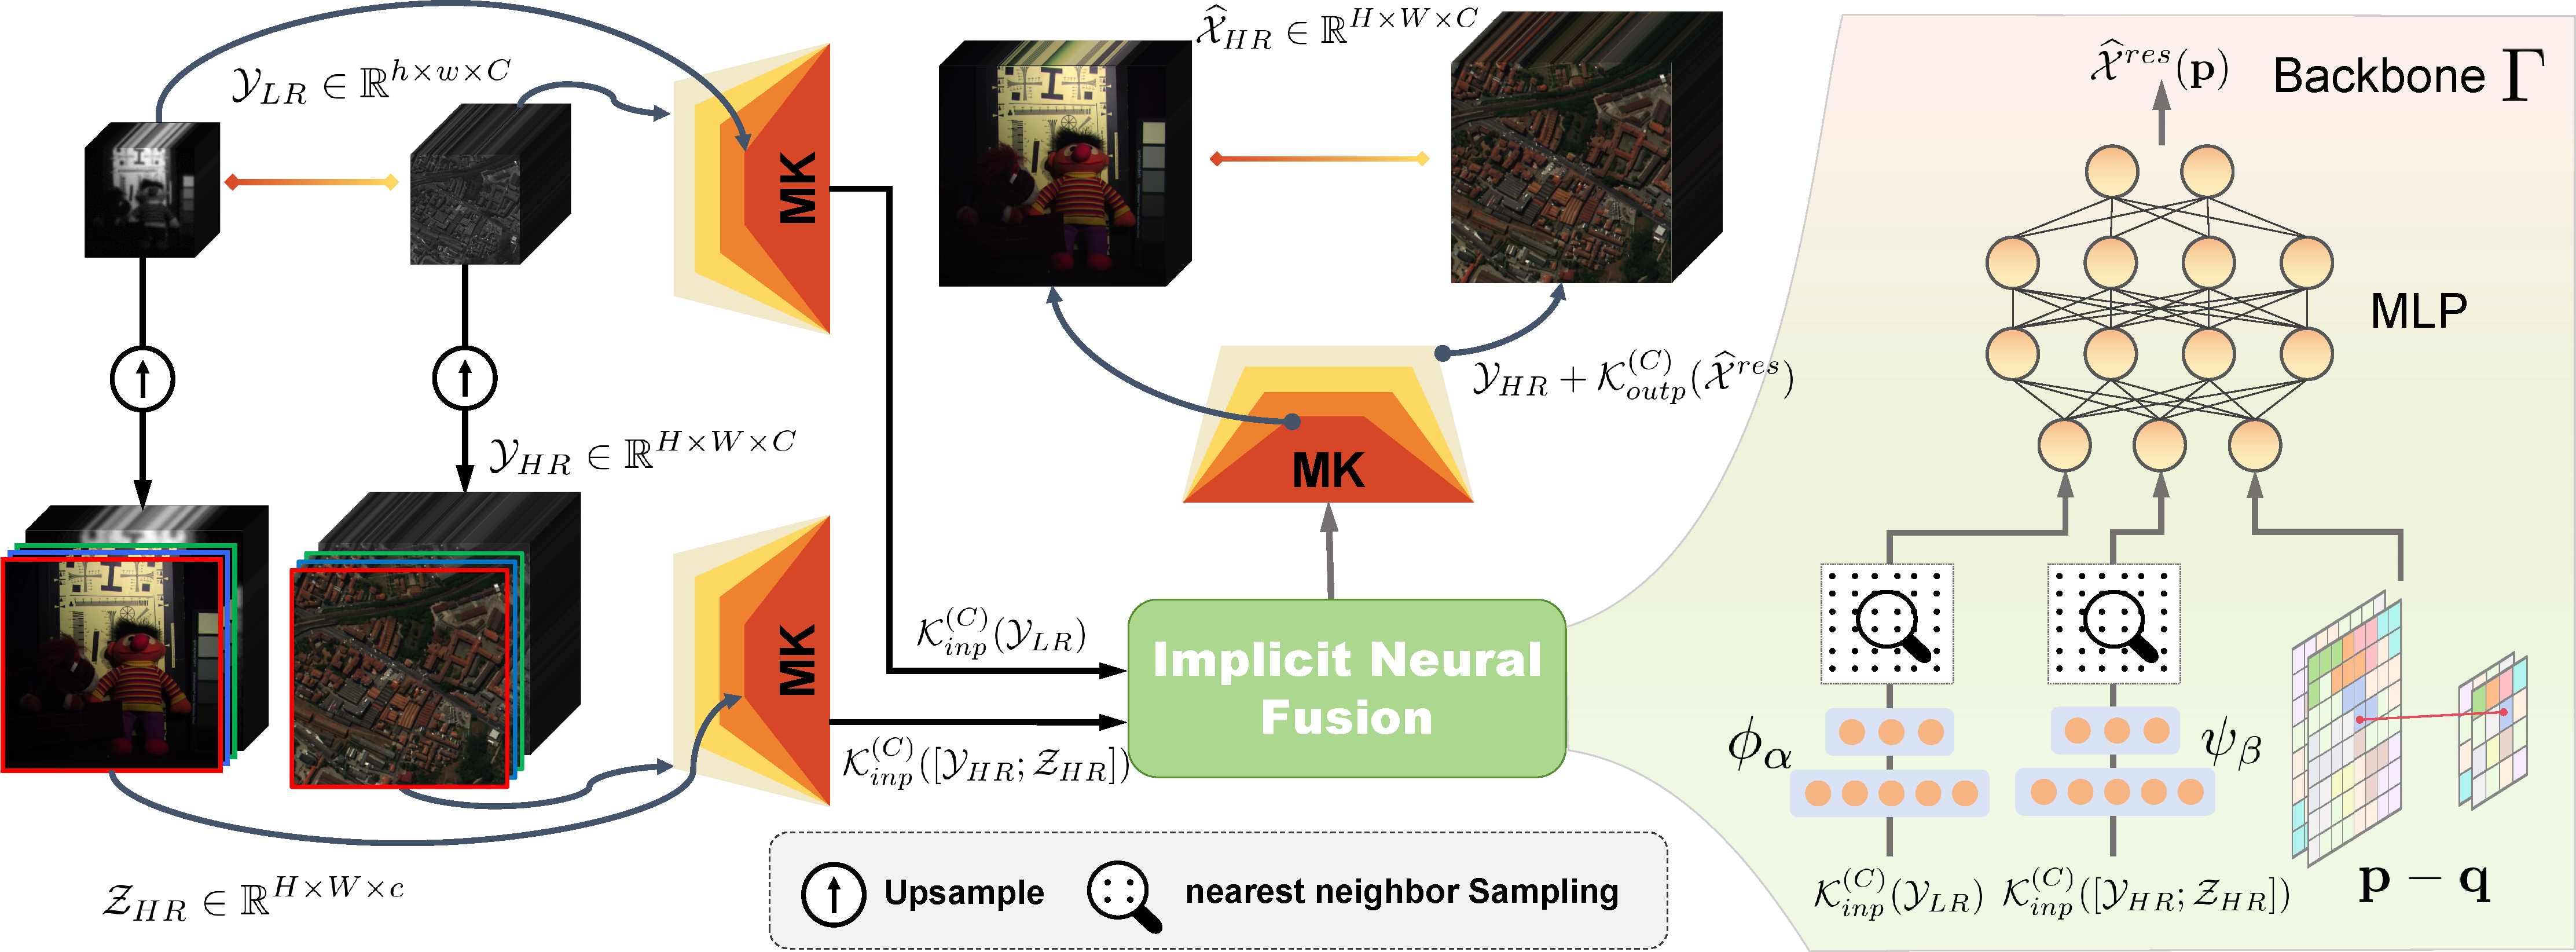
\includegraphics[width=\textwidth]{Figs/pipeline.pdf}
    \caption{The overall architecture of our proposed SSA framework. This end-to-end model realizes the universal mapping function $\mathcal{F}$, which takes an LR-HSI and an HR-MSI from \textit{various sensors} as input and reconstructs a high-fidelity HR-HSI at \textit{arbitrary scales}.}
    \label{fig: architecture}
\end{figure*}

Recently, several works~\cite{zhang2022implicit,chen2023spectral} have begun to apply Implicit Neural Representation (INR) to HSI data, modeling the image as a continuous function of coordinates. This approach enables reconstruction at arbitrary scales, neatly addressing the spatial rigidity of conventional models. Subsequent research has explored various extensions, such as integrating low-rank properties~\cite{wang2025hyperspectral}, performing fusion in the frequency domain~\cite{liang2024fourier}, or using adaptive sampling~\cite{deng2025otias}. However, despite solving spatial rigidity, these methods face two key limitations: First, they lack spectral flexibility, as models must be re-engineered for datasets with different numbers of bands. Second, as data-driven approaches, achieving strong generalization can be difficult given the limited volume of available HSI data.

\subsection{Matryoshka Representation Learning and Flexible Model Design}
Our solution is philosophically inspired by the broader trend in machine learning towards building more adaptive and general-purpose models. From the perspective of representation granularity adaptation, Matryoshka Representation Learning (MRL)~\cite{kusupati2022matryoshka,hojjat2025thinkingvit,cappellazzo2025mome} was proposed to explore model flexibility. The core idea of MRL is to train a single, high-dimensional feature vector $z \in \mathbb R^d$ that encodes information at different granularities in a nested fashion, such that its shorter prefixes also serve as valid representations. This paradigm provides flexible representations for downstream tasks with varying computational demands.

Formally, a nested representation $z$ obtained by a deep neural network $z:=F(\cdot,\theta_F): \mathcal X\to \mathbb R^d$ contains different granularities representations: $z_{1:m}\in \mathbb R^m$, where $m$ is the desired dimension and $(r:s)$ means one sub-representation choosing algorithm. The Matryoshka representation is acquired to minimize the empirical risk (that is, a valid representation). Under the classification context and parameterizing the nested $z$ as the classifier weights $\mathbf W^{(m)} \in \mathbb R^{N, m}$, the expirical risk can be supervised using cross-entropy loss:
\begin{equation}
    \min_{\substack{\theta_F, \\ \{\mathbf W^{(m)}\}_{\substack{m\in \mathcal M, \\ m\leq d}}}}\frac{1}{N} \sum_{m \in \mathcal M} \mathcal L\left(\mathbf W^{(m)} \cdot F(x,\theta_F)_{1:m}; y \right), \label{eq:mrl-loss}
\end{equation}
where $\mathcal M$ is a nested chosen list (\textit{e.g,} $\mathcal M:=\{m_1,\dots,m_i,d\}$, $m_1\leq m_i\leq d$), $N$ is the total classification number, $(x,y)$ is the data/label pair. In the MRL paper, the sub-representation choosing algorithm is designed as dim-slicing, where $r$ is fixed to 1 and $s=m$.

% enabling adaptive deployment per computational constraints.
% This representation strategy has recently received widespread attention, with many works leveraging shared models to construct embeddings of different granularities. For example, ThinkingViT~\cite{hojjat2025thinkingvit} integrates a nested structure to dynamically adjust its computational budget based on input image complexity. MoME~\cite{cappellazzo2025mome} combines MRL with Mixture-of-Experts for audio-visual speech recognition. MatryoshkaKV~\cite{lin2024matryoshkakv} introduces an adaptive method that compresses the key-value cache along the feature dimension in large language models through trainable orthogonal projections and a Matryoshka-style training strategy. fMRLRec~\cite{wang2024train} utilizes linear recurrent units and a full-scale Matryoshka operator to fuse text and image features, learning item representations of multiple granularities in a single training run.

% The principle of achieving flexibility through a nested, structured representation, as demonstrated by MRL, provides powerful inspiration for our work. 
Different from the MRL, which aims at learning flexible valid representation, and inference with different size model dimension~\cite{lin2024matryoshkakv,wang2024train}, we bring the nested principle into the hyperspectral data fusion kernels to handle various input image channels, termed as Matryoshka Kernels (MK, see \S  \ref{subsec:mk}).
This convertion eliminates  previous two key drawbacks: architectural rigidity, data scarity, and model scale.  

% We term this architectural innovation Matryoshka Kernels (MK). Unlike MRL, which creates nested embeddings, our spectral-agnostic layers create nested convolutional kernels. This allows the model architecture itself to dynamically and non-parametrically adapt to a fundamental property of the input data—namely, its number of spectral channels. This architectural adaptability offers a direct solution to the problem of input structural heterogeneity.

% In summary, SA$^2$ is the first framework to synergize the established spatial flexibility of the INR paradigm with the novel spectral flexibility afforded by our proposed Matryoshka Kernels. By doing so, it overcomes a core limitation of prior HSI-SR approaches and lays the groundwork for the development of a general-purpose foundation model for hyperspectral image analysis.

